%==============================================================
%  EE201 -- Circuit Theory I
%  Lecture 17 : Capacitors -- slides
%  M. Mert Ankaralı, METU EEE
%
%  Compile:  ./build.sh      (or: pdflatex EE201_Lecture_16_slides.tex, twice)
%  Same colour code as the handout:
%      charge = purple, current = blue, voltage = orange, power = green
%==============================================================
\documentclass[11pt,aspectratio=169]{beamer}

\usepackage{appendixnumberbeamer}
\usepackage[T1]{fontenc}
\usepackage[utf8]{inputenc}
\usepackage[english]{babel}
\usepackage{lmodern}
\usepackage{amsmath,amssymb}
\usepackage{booktabs}
\usepackage{array}
\usepackage{colortbl}
\usepackage{tikz}
\usepackage[american,siunitx]{circuitikz}
\usetikzlibrary{matrix,arrows.meta,positioning,calc,decorations.pathreplacing,decorations.pathmorphing,decorations.markings}
\usetikzlibrary{overlay-beamer-styles}

%-------------------- plain METU-flavoured theme --------------
\usetheme{default}
\usecolortheme{default}
\useinnertheme{rectangles}
\setbeamertemplate{navigation symbols}{}
\setbeamertemplate{itemize items}[square]
\setbeamerfont{frametitle}{size=\large,series=\bfseries}
\setbeamerfont{title}{size=\LARGE,series=\bfseries}

\definecolor{metured}{RGB}{155,27,48}
\definecolor{metugray}{RGB}{88,89,91}
\definecolor{metulight}{RGB}{243,240,241}
\definecolor{ccur}{RGB}{0,102,170}
\definecolor{cvolt}{RGB}{214,120,0}
\definecolor{cpow}{RGB}{23,128,74}
\definecolor{ccharge}{RGB}{124,60,160}
\definecolor{cflux}{RGB}{0,138,138}
\definecolor{copper}{RGB}{184,98,30}

\setbeamercolor{structure}{fg=metured}
\setbeamercolor{frametitle}{fg=metured,bg=}
\setbeamercolor{title}{fg=metured}
\setbeamercolor{normal text}{fg=black!88}
\setbeamercolor{block title}{fg=white,bg=metured}
\setbeamercolor{block body}{bg=metulight}
\setbeamercolor{alerted text}{fg=metured}

\setbeamertemplate{frametitle}{%
  \vspace{0.55em}%
  \usebeamerfont{frametitle}\usebeamercolor[fg]{frametitle}\insertframetitle\par
  \vspace{-0.2em}{\color{metured}\rule{\textwidth}{1pt}}\par\vspace{-0.2em}}

\setbeamertemplate{footline}{%
  \hbox{\begin{beamercolorbox}[wd=\paperwidth,ht=2.4ex,dp=1.4ex,leftskip=1.2em,rightskip=1.2em]{}%
  \tiny\color{metugray}\coursecode\ \textbar\ Lecture 17: Capacitors
  \hfill \insertframenumber/\inserttotalframenumber
  \end{beamercolorbox}}}

%-------------------- macros ----------------------------------
\newcommand{\coursecode}{EE201}
\newcommand{\term}{Fall 2026--2027}
\newcommand{\Icol}[1]{\textcolor{ccur}{#1}}
\newcommand{\Vcol}[1]{\textcolor{cvolt}{#1}}
\newcommand{\Pcol}[1]{\textcolor{cpow}{#1}}
\newcommand{\Qcol}[1]{\textcolor{ccharge}{#1}}
\newcommand{\Fcol}[1]{\textcolor{cflux}{#1}}
\newcommand{\uni}[1]{\,\mathrm{#1}}
\newcommand{\A}{\uni{A}} \newcommand{\V}{\uni{V}}
\newcommand{\W}{\uni{W}} \newcommand{\J}{\uni{J}}
\newcommand{\Cb}{\uni{C}} \newcommand{\s}{\uni{s}}
\newcommand{\Wb}{\uni{Wb}} \newcommand{\Hy}{\uni{H}}
\newcommand{\Sie}{\uni{S}}


%  voltage sources: smaller + and - inside the circle, further apart
\ctikzset{bipoles/vsourceam/inner plus={\tiny$+$},
          bipoles/vsourceam/inner minus={\tiny$\vphantom{+}-$},
          bipoles/vsourceam/margin=0.85,
          bipoles/cvsourceam/inner plus={\tiny$+$},
          bipoles/cvsourceam/inner minus={\tiny$\vphantom{+}-$},
          bipoles/cvsourceam/margin=0.85}
\ctikzset{bipoles/length=0.9cm, label/align=straight,
          bipoles/generic/height=0.28, bipoles/generic/width=0.62}
\tikzset{
  iar/.style={-{Stealth[length=2.2mm]}, ccur, thick},
  glab/.style={font=\footnotesize, text=metured},
  ttl/.style={font=\scriptsize\bfseries, text=metugray},
  capn/.style={font=\scriptsize, text=metugray, align=center},
  pol/.style={font=\small, text=cvolt},
  nlab/.style={circle, draw=metured, text=metured, font=\scriptsize, inner sep=0.7pt},
  blab/.style={font=\footnotesize, text=black!80},
  gbr/.style={black!75, thick, postaction={decorate, decoration={markings,
      mark=at position 0.56 with {\arrow{Stealth[length=2.5mm]}}}}},
  hal/.style={draw=cpow!60, line width=6pt, opacity=0.35, line cap=round, line join=round},
  halo/.style={circle, fill=metured!16, minimum size=0.95cm},
  elem/.style={draw=metugray, thick, fill=metulight},
  bigarr/.style={-{Stealth[length=3mm]}, very thick, metugray},
}

%-------------------- Lecture 15 circuit macros ---------------
%-------------------- Lecture 17 macros: capacitors ---------------
\newcommand{\ohm}{\,\Omega}
\newcommand{\F}{\,\mathrm{F}}
\newcommand{\Jl}{\,\mathrm{J}}
\newcommand{\yes}{\textcolor{cpow}{\checkmark}}
\newcommand{\vC}{\Vcol{v_C}}
\newcommand{\iC}{\Icol{i_C}}
\newcommand{\iR}{\Icol{i_R}}
\newcommand{\Vo}{V_0}
\newcommand{\zm}{0^-}
\newcommand{\zp}{0^+}
\tikzset{vax/.style={-{Stealth[length=2mm]}, gray!70},
         crv/.style={metured, very thick, line join=round},
         crvu/.style={metured, very thick, dashed, line join=round},
         gdash/.style={black!45, densely dashed, thin},
         reg/.style={font=\scriptsize, text=metugray, align=center},
         imp/.style={metured, very thick, -{Stealth[length=2.6mm, width=2.4mm]}}}
%  axes and ticks in data units
\newcommand{\tax}[6]{\draw[vax] (#1,0) -- (#2,0) node[right, font=\small] {#5};
  \draw[vax] (0,#3) -- (0,#4) node[above, font=\small] {#6};}
\newcommand{\xt}[2]{\draw ([yshift=2pt]#1,0) -- ([yshift=-2pt]#1,0) node[below, font=\scriptsize] {#2};}
\newcommand{\xtu}[2]{\draw ([yshift=2pt]#1,0) -- ([yshift=-2pt]#1,0); \node[above, font=\scriptsize] at (#1,0) {#2};}
\newcommand{\yt}[2]{\draw ([xshift=2pt]0,#1) -- ([xshift=-2pt]0,#1) node[left, font=\scriptsize] {#2};}
\newcommand{\ytr}[2]{\draw ([xshift=2pt]0,#1) -- ([xshift=-2pt]0,#1); \node[right, font=\scriptsize] at (0,#1) {#2};}

%  ---------- singularity functions ----------
\newcommand{\stepPlot}{%
  \tax{-1.2}{2.4}{-0.3}{1.6}{$t$}{$u(t)$}
  \draw[crv] (-1.1,0) -- (0,0); \draw[crv] (0,1) -- (2.2,1); \yt{1}{$1$}}
\newcommand{\rampPlot}{%
  \tax{-1.2}{2.4}{-0.3}{1.9}{$t$}{$r(t)$}
  \draw[crv] (-1.1,0) -- (0,0) -- (1.7,1.7);
  \draw[gdash] (1,0) -- (1,1); \xt{1}{$1$}
  \node[font=\scriptsize, anchor=west] at (1.05,0.7) {slope $1$};}
\newcommand{\impPlot}{%
  \tax{-1.2}{2.4}{-0.3}{1.6}{$t$}{$\delta(t)$}
  \draw[crv] (-1.1,0) -- (2.2,0);
  \draw[imp] (0,0) -- (0,1.1); \node[font=\scriptsize, anchor=west] at (0.05,1.05) {$(1)$};}
\newcommand{\pulsePlot}{%
  \tax{-1.2}{2.4}{-0.3}{2.3}{$t$}{}
  \draw[crv] (-1.1,0) -- (0,0) -- (0,1.8) -- (0.6,1.8) -- (0.6,0) -- (2.2,0);
  \xt{0.6}{$\Delta$} \yt{1.8}{$1/\Delta$}
  \node[font=\scriptsize, anchor=west] at (0.7,1.5) {area $1$};}

%  ---------- the capacitor ----------
\newcommand{\capDef}{%
  \draw (0,2.2) node[ocirc] {} to[C, l=$C$, i>^=$\Icol{i}$] (0,0) node[ocirc] {};
  \node[pol] at (-0.55,1.85) {$+$}; \node[pol] at (-0.55,0.35) {$-$};
  \node[font=\small, text=cvolt] at (-0.6,1.1) {$v$};}
%  initial-condition models: #1 = 1, 2 or 3
\newcommand{\icModel}[1]{%
  \ifcase#1\or
    \draw (0,2.4) node[ocirc] {} to[C, l=$C$] (0,0) node[ocirc] {};
    \node[pol] at (-0.5,2.0) {$+$}; \node[pol] at (-0.5,0.4) {$-$};
    \node[font=\small, text=cvolt] at (-0.6,1.2) {$v$};
    \node[font=\scriptsize, align=center] at (0,-0.55) {$v(t_0^-) = \Vo$};
  \or
    \draw (0,2.4) node[ocirc] {} to[C, l=$C$] (0,1.2) to[american voltage source, l=$\Vo\,u(t - t_0)$] (0,-0.4) node[ocirc] {};
    \node[pol] at (-0.5,2.0) {$+$}; \node[pol] at (-0.5,0) {$-$};
    \node[font=\small, text=cvolt] at (-0.6,1.0) {$v$};
    \node[font=\scriptsize, align=center] at (0,-0.95) {uncharged};
  \or
    \draw (0,2.4) node[ocirc] {} -- (2.9,2.4); \draw (0,0) node[ocirc] {} -- (2.9,0);
    \draw (1.0,2.4) to[C, l=$C$] (1.0,0);
    \draw (2.9,0) to[american current source, l_=$C\Vo\,\delta(t - t_0)$] (2.9,2.4);
    \fill (1.0,0) circle (1.6pt); \fill (1.0,2.4) circle (1.6pt);
    \node[pol] at (-0.35,2.0) {$+$}; \node[pol] at (-0.35,0.4) {$-$};
    \node[font=\small, text=cvolt] at (-0.4,1.2) {$v$};
    \node[font=\scriptsize, align=center] at (1.4,-0.55) {uncharged};
  \fi}
%  parallel and series connections
\newcommand{\capPar}{%
  \draw (0,2) node[ocirc] {} -- (5.0,2); \draw (0,0) node[ocirc] {} -- (5.0,0);
  \draw (1.0,2) to[C, l=$C_1$] (1.0,0); \draw (2.4,2) to[C, l=$C_2$] (2.4,0);
  \node at (3.9,1) {$\cdots$}; \draw (5.0,2) to[C, l=$C_n$] (5.0,0);
  \fill (1.0,2) circle (1.6pt); \fill (2.4,2) circle (1.6pt); \fill (1.0,0) circle (1.6pt); \fill (2.4,0) circle (1.6pt);
  \node[pol] at (-0.3,1.7) {$+$}; \node[pol] at (-0.3,0.3) {$-$}; \node[font=\small, text=cvolt] at (-0.35,1) {$v$};}
\newcommand{\capSer}{%
  \draw (0,2) node[ocirc] {} to[C, l=$C_1$] (1.6,2) to[C, l=$C_2$] (3.2,2) -- (3.6,2);
  \node at (4.0,2) {$\cdots$};
  \draw (4.4,2) to[C, l=$C_n$] (5.8,2) -- (5.8,0) -- (0,0) node[ocirc] {};
  \node[pol] at (-0.3,1.7) {$+$}; \node[pol] at (-0.3,0.3) {$-$}; \node[font=\small, text=cvolt] at (-0.35,1) {$v$};}
%  current division: source i_s feeding C1 || C2
\newcommand{\cdiv}{%
  \draw (0,0) to[american current source, l=$\Icol{i_s}$] (0,2) -- (3.2,2);
  \draw (1.6,2) to[C, l=$C_1$, i>^=$\Icol{i_1}$] (1.6,0);
  \draw (3.2,2) to[C, l=$C_2$, i>^=$\Icol{i_2}$] (3.2,0) -- (0,0);
  \fill (1.6,2) circle (1.6pt); \fill (1.6,0) circle (1.6pt);}
%  voltage division: source, switch, C1 and C2 in series
\newcommand{\vdiv}{%
  \draw (0,0) to[american voltage source, l=$\Vcol{v_s}$, invert] (0,2.6) -- (1.8,2.6) to[cspst, l={$t = 0$}] (3.2,2.6) -- (3.2,2.5);
  \draw (3.2,2.5) to[C, l_=$C_1$] (3.2,1.3) to[C, l_=$C_2$] (3.2,0.1) -- (3.2,0) -- (0,0);
  \node[pol] at (3.75,2.3) {$+$}; \node[pol] at (3.75,1.5) {$-$}; \node[font=\small, text=cvolt] at (3.8,1.9) {$v_1$};
  \node[pol] at (3.75,1.1) {$+$}; \node[pol] at (3.75,0.3) {$-$}; \node[font=\small, text=cvolt] at (3.8,0.7) {$v_2$};}
%  parallel RC driven by a current source: #1 source label, #2 R, #3 C
\newcommand{\rcPar}[3]{%
  \draw (0,0) to[american current source, l=#1] (0,2.2) -- (3.6,2.2);
  \draw (1.8,2.2) to[R, l_=#2, i>^=$\iR$] (1.8,0);
  \draw (3.6,2.2) to[C, l=#3, i>^=$\iC$] (3.6,0) -- (0,0);
  \fill (1.8,2.2) circle (1.6pt); \fill (1.8,0) circle (1.6pt);
  \node[pol] at (2.75,1.85) {$+$}; \node[pol] at (2.75,0.35) {$-$}; \node[font=\small, text=cvolt] at (2.75,1.1) {$v_C$};}
%  capacitor discharged through a resistor at t = 0
\newcommand{\rcDis}{%
  \draw (0,0) to[C, l_=$C$] (0,2.2) -- (0.8,2.2) to[cspst, l={$t = 0$}] (2.2,2.2) -- (3.0,2.2) to[R, l=$R$, i>^=$\iR$] (3.0,0) -- (0,0);
  \node[pol] at (-0.5,1.85) {$+$}; \node[pol] at (-0.5,0.35) {$-$}; \node[font=\small, text=cvolt] at (-0.6,1.1) {$v_C$};}
%  two capacitors connected by a switch at t = 0
\newcommand{\twoCap}{%
  \draw (0,0) to[C, l_=$3\F$] (0,2.2) -- (0.8,2.2) to[cspst, l={$t = 0$}] (2.2,2.2) -- (3.0,2.2) to[C, l_=$6\F$] (3.0,0) -- (0,0);
  \node[pol] at (-0.5,1.85) {$+$}; \node[pol] at (-0.5,0.35) {$-$}; \node[font=\small, text=cvolt] at (-0.6,1.1) {$v_1$};
  \node[pol] at (3.55,1.85) {$+$}; \node[pol] at (3.55,0.35) {$-$}; \node[font=\small, text=cvolt] at (3.6,1.1) {$v_2$};}
\title{Lecture 17: Capacitors}
\subtitle{EE201 -- Circuit Theory I}
\author{M. Mert Ankaral{\i}}
\institute{\small Department of Electrical and Electronics Engineering\\
           Middle East Technical University}
\date{}

%  Roadmap icons (1-6)
\newcommand{\rmicon}[1]{%
  \ifcase#1\or
    \draw[-{Stealth[length=2mm]}] (-1.5,0) -- (1.7,0); \draw[-{Stealth[length=2mm]}] (-0.6,-0.3) -- (-0.6,1.6);
    \draw[metured, very thick] (-1.4,0) -- (0,0) -- (0,0.8) -- (1.5,0.8);
    \draw[metured, very thick, -{Stealth[length=2.4mm]}] (-0.6,0) -- (-0.6,1.25);
  \or
    \draw (0,1.3) node[ocirc] {} to[C] (0,-1.3) node[ocirc] {};
    \draw[-{Stealth[length=2.4mm]}, ccur, thick] (0.35,1.2) -- (0.35,0.6);
  \or
    \draw (0,1.6) node[ocirc] {} to[C] (0,0.2) to[american voltage source] (0,-1.4) node[ocirc] {};
  \or
    \draw (-1.4,1.2) node[ocirc] {} -- (1.4,1.2); \draw (-1.4,-1.2) node[ocirc] {} -- (1.4,-1.2);
    \draw (-0.3,1.2) to[C] (-0.3,-1.2); \draw (1.0,1.2) to[C] (1.0,-1.2);
  \or
    \draw (-1.2,-1.1) to[american current source] (-1.2,1.1) -- (1.2,1.1) to[C] (1.2,-1.1) -- (-1.2,-1.1);
  \or
    \draw[-{Stealth[length=2mm]}] (-1.4,0) -- (1.8,0); \draw[-{Stealth[length=2mm]}] (-1.2,-0.3) -- (-1.2,1.7);
    \draw[metured, very thick, domain=0:2.8, samples=40] plot ({-1.2+\x}, {1.3*exp(-1.3*\x)});
  \fi}
%  Stops 1-12: station of stop k = \rmst{k}
\newcommand{\rmst}[1]{\ifcase#1\or1\or1\or1\or2\or2\or3\or4\or4\or5\or5\or6\or6\fi}
\newcommand{\rmstation}[4]{%
  \ifnum#1<\rmS\relax
    \node[circle, fill=cpow, text=white, inner sep=0pt, minimum size=5.4mm, font=\scriptsize\bfseries] at (#2,0) {\checkmark};
    \node[text=black!40, font=\footnotesize\bfseries, align=center, anchor=south, inner sep=1pt] at (#2,0.36) {#3};
  \else\ifnum#1=\rmS\relax
    \node[circle, fill=metured, text=white, inner sep=0pt, minimum size=6.2mm, font=\small\bfseries] at (#2,0) {#1};
    \node[text=metured, font=\footnotesize\bfseries, align=center, anchor=south, inner sep=1pt] at (#2,0.36) {#3};
  \else
    \node[circle, draw=metugray, fill=white, text=metugray, inner sep=0pt, minimum size=5.4mm, font=\scriptsize\bfseries] at (#2,0) {#1};
    \node[font=\footnotesize\bfseries, align=center, anchor=south, inner sep=1pt] at (#2,0.36) {#3};
  \fi\fi
  \begin{scope}[shift={(#2,1.75)}, scale=0.34, transform shape]
    \ifnum#1>\rmS\relax\begin{scope}[opacity=0.5]\rmicon{#4}\end{scope}\else\rmicon{#4}\fi
  \end{scope}}
%  #1 first stop, #2 last stop covered by this item, #3 x, #4 y, #5 text
\newcommand{\rmsub}[5]{%
  \ifnum#2<\rmcur\relax
    \node[text width=1.95cm, align=center, font=\scriptsize, text=black!40] at (#3,#4) {#5\ \textcolor{cpow}{\checkmark}};
  \else\ifnum#1>\rmcur\relax
    \node[text width=1.95cm, align=center, font=\scriptsize] at (#3,#4) {#5};
  \else
    \node[text width=1.95cm, align=center, font=\scriptsize\bfseries, text=metured,
          draw=metured, rounded corners=2pt, inner sep=2pt] at (#3,#4) {#5};
  \fi\fi}
\newcommand{\roadmapframe}[1]{%
  \begin{frame}{Roadmap}
    \def\rmcur{#1}\edef\rmS{\rmst{#1}}%
    \vfill
    \centering
    \begin{tikzpicture}
      \draw[metugray!45, line width=3pt, -{Stealth[length=2.6mm, width=3.2mm]}] (0,0) -- (13.4,0);
      \rmstation{1}{1.20}{Singularity\\ functions}{1}
      \rmstation{2}{3.40}{The\\ capacitor}{2}
      \rmstation{3}{5.60}{Initial\\ conditions}{3}
      \rmstation{4}{7.80}{Connections}{4}
      \rmstation{5}{10.00}{From $0^-$\\ to $0^+$}{5}
      \rmstation{6}{12.20}{Energy\\ examples}{6}
      \rmsub{1}{1}{1.20}{-0.8}{step, ramp, impulse}
      \rmsub{2}{2}{1.20}{-1.5}{sketches, derivatives}
      \rmsub{3}{3}{1.20}{-2.1}{sifting}
      \rmsub{4}{4}{3.40}{-0.8}{$i = C\,dv/dt$}
      \rmsub{5}{5}{3.40}{-1.5}{energy}
      \rmsub{6}{6}{5.60}{-0.8}{three models}
      \rmsub{7}{7}{7.80}{-0.8}{parallel, series}
      \rmsub{8}{8}{7.80}{-1.6}{division}
      \rmsub{9}{9}{10.00}{-0.8}{continuity}
      \rmsub{10}{10}{10.00}{-1.5}{impulsive current}
      \rmsub{11}{11}{12.20}{-0.8}{RC discharge}
      \rmsub{12}{12}{12.20}{-1.5}{two capacitors}
    \end{tikzpicture}
    \vfill
    \mbox{}
    \vfill
  \end{frame}}
\newcommand{\qbox}[1]{\begin{tikzpicture}\node[draw=metured, thick, fill=metured!5, rounded corners=3pt, inner sep=5pt] {#1};\end{tikzpicture}}

\begin{document}

%--------------------------------------------------------------
\begin{frame}[plain]
  \titlepage
  \vspace{-1.2em}
  \begin{center}\scriptsize\color{metugray}
    \Icol{$\blacksquare$}~current \quad \Vcol{$\blacksquare$}~voltage \quad
    \Pcol{$\blacksquare$}~energy \quad \textcolor{metured}{$\blacksquare$}~waveform
  \end{center}
\end{frame}

%--------------------------------------------------------------
\begin{frame}{Motivation: an element with memory}
  \vfill
  \begin{columns}[c,onlytextwidth]
    \begin{column}{0.42\textwidth}
      \centering
      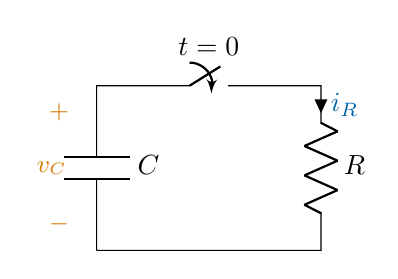
\begin{tikzpicture}[scale=0.95]\rcDis\end{tikzpicture}
    \end{column}
    \begin{column}{0.56\textwidth}
      \begin{itemize}\itemsep8pt
        \item Resistor: $v(t)$ depends only on $i(t)$ now \ (no memory)
        \item Capacitor: current depends on \emph{how fast} $v$ changes
        \item It stores energy and remembers its past
        \item Switches act at an instant: we need step, ramp and impulse
      \end{itemize}
    \end{column}
  \end{columns}
  \vfill
\end{frame}

%==============================================================
\roadmapframe{1}

%--------------------------------------------------------------
\begin{frame}{Step, ramp and impulse}
  \vfill
  \centering
  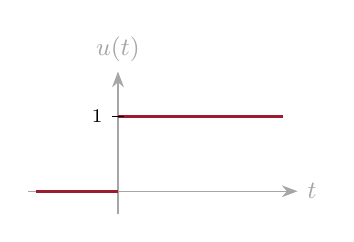
\begin{tikzpicture}[x=0.95cm,y=0.95cm]\stepPlot\end{tikzpicture}\hfill
  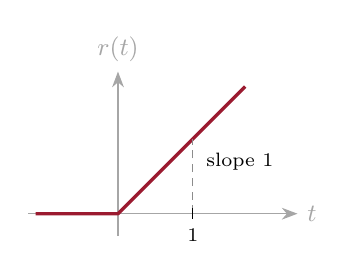
\begin{tikzpicture}[x=0.95cm,y=0.95cm]\rampPlot\end{tikzpicture}\hfill
  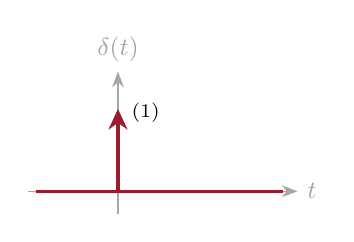
\begin{tikzpicture}[x=0.95cm,y=0.95cm]\impPlot\end{tikzpicture}
  \vfill
  \[
    u(t) = \begin{cases} 1, & t > 0\\ 0, & t < 0 \end{cases}
    \qquad\qquad
    r(t) = \begin{cases} t, & t \geq 0\\ 0, & t < 0 \end{cases}
    \qquad\qquad
    \delta(t)\ :\ \text{an arrow of area } 1
  \]
  \vfill
\end{frame}

%--------------------------------------------------------------
\begin{frame}{The unit impulse as a limit}
  \vfill
  \begin{columns}[c,onlytextwidth]
    \begin{column}{0.4\textwidth}
      \centering
      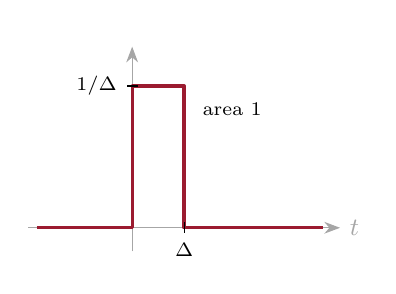
\begin{tikzpicture}[x=1.1cm,y=1.0cm]\pulsePlot\end{tikzpicture}
    \end{column}
    \begin{column}{0.58\textwidth}
      \[
        \delta(t) = \lim_{\Delta \to 0} \frac{u(t) - u(t - \Delta)}{\Delta}
      \]
      \begin{itemize}\itemsep6pt
        \item Area $1$ for every $\Delta$; narrower and taller
        \item $\delta(t) = 0$ for $t \neq 0$, \ $\displaystyle\int_{-\alpha}^{\beta} \delta\,dt = 1$
      \end{itemize}
    \end{column}
  \end{columns}
  \vfill
  \pause
  \centering
  \qbox{$\displaystyle \int_{-\infty}^{t} \delta\,d\tau = u(t), \quad \int_{-\infty}^{t} u\,d\tau = r(t), \quad
    \frac{d}{dt}r = u, \quad \frac{d}{dt}u = \delta$}\\[6pt]
  \small A jump of size $a$ at $t_0$ gives $a\,\delta(t - t_0)$ in the derivative.
  \vfill
\end{frame}

%==============================================================
\roadmapframe{2}

%--------------------------------------------------------------
\begin{frame}{Example 17.1 and 17.2: formula $\leftrightarrow$ sketch}
  \begin{columns}[t,onlytextwidth]
    \begin{column}{0.48\textwidth}
      \textbf{Sketch} $f(t) = 2\,u(-t - 1)$.\\[10pt]
      \onslide<2->{%
        $s = -t - 1 > 0 \iff t < -1$\\[8pt]
        \centering
        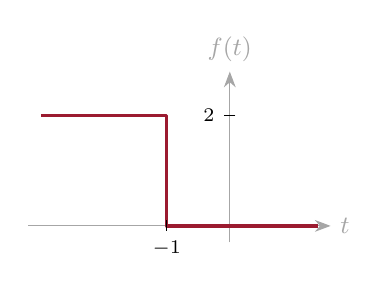
\begin{tikzpicture}[x=0.8cm,y=0.7cm]
          \tax{-3.2}{1.6}{-0.3}{2.8}{$t$}{$f(t)$}
          \draw[crv] (-3.0,2) -- (-1,2) -- (-1,0) -- (1.4,0);
          \xt{-1}{$-1$} \yt{2}{$2$}
        \end{tikzpicture}\\[4pt]
        \small The minus sign flips the step.}
    \end{column}
    \begin{column}{0.5\textwidth}
      \textbf{Write} the triangle with ramps.\\[4pt]
      \centering
      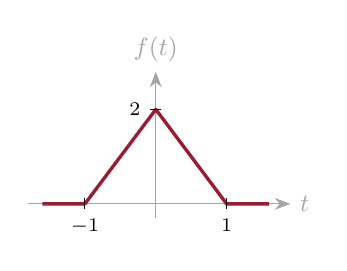
\begin{tikzpicture}[x=0.9cm,y=0.6cm]
        \tax{-1.8}{1.9}{-0.3}{2.8}{$t$}{$f(t)$}
        \draw[crv] (-1.6,0) -- (-1,0) -- (0,2) -- (1,0) -- (1.6,0);
        \xt{-1}{$-1$} \xt{1}{$1$} \yt{2}{$2$}
      \end{tikzpicture}\\[4pt]
      \raggedright\small
      \onslide<3->{Slope changes: $+2$ at $-1$, \ $-4$ at $0$, \ $+2$ at $1$\\[6pt]}
      \onslide<4->{\centering\qbox{$f(t) = 2r(t + 1) - 4r(t) + 2r(t - 1)$}}
    \end{column}
  \end{columns}
\end{frame}

%--------------------------------------------------------------
\begin{frame}{Example 17.3: derivatives give impulses}
  \begin{columns}[c,onlytextwidth]
    \begin{column}{0.44\textwidth}
      \centering
      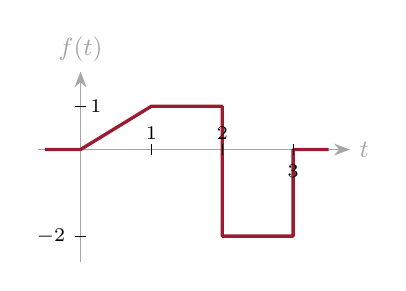
\begin{tikzpicture}[x=0.9cm,y=0.55cm]
        \tax{-0.6}{3.8}{-2.6}{1.8}{$t$}{$f(t)$}
        \draw[crv] (-0.5,0) -- (0,0) -- (1,1) -- (2,1) -- (2,-2) -- (3,-2) -- (3,0) -- (3.5,0);
        \xtu{1}{$1$} \xtu{2}{$2$} \xt{3}{$3$} \ytr{1}{$1$} \yt{-2}{$-2$}
      \end{tikzpicture}\\[2pt]
      \onslide<3->{%
      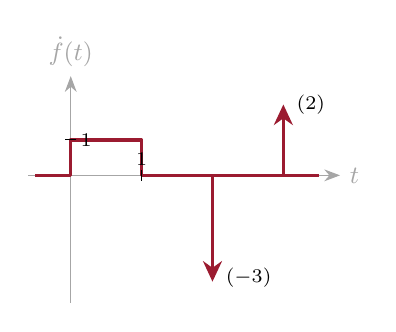
\begin{tikzpicture}[x=0.9cm,y=0.45cm]
        \tax{-0.6}{3.8}{-3.6}{2.8}{$t$}{$\dot f(t)$}
        \draw[crv] (-0.5,0) -- (0,0) -- (0,1) -- (1,1) -- (1,0) -- (3.5,0);
        \draw[imp] (2,0) -- (2,-3); \node[font=\scriptsize, anchor=west] at (2.05,-2.9) {$(-3)$};
        \draw[imp] (3,0) -- (3,2); \node[font=\scriptsize, anchor=west] at (3.05,2.0) {$(2)$};
        \xtu{1}{$1$} \ytr{1}{$1$}
      \end{tikzpicture}}
    \end{column}
    \begin{column}{0.54\textwidth}
      Write $f$ with ramps and steps; find $\dot f$.\\[10pt]
      \onslide<2->{Ramp on $[0,1]$, jump $-3$ at $2$, jump $+2$ at $3$:
        \[ f = r(t) - r(t - 1) - 3u(t - 2) + 2u(t - 3) \]}
      \onslide<3->{\[ \dot f = u(t) - u(t - 1) - 3\delta(t - 2) + 2\delta(t - 3) \]
        \small Each jump gives an impulse with area = jump size.}
    \end{column}
  \end{columns}
\end{frame}

%==============================================================
\roadmapframe{3}

%--------------------------------------------------------------
\begin{frame}{The sifting property}
  \vfill
  Only $f(0)$ matters, since $\delta(t) = 0$ for $t \neq 0$:
  \[
    \int_{-T}^{T} f(t)\,\delta(t)\,dt = f(0) \qquad (T > 0)
  \]
  \pause
  With the pulse:
  \[
    \int f(t)\,\frac{u(t) - u(t - \Delta)}{\Delta}\,dt = \frac{1}{\Delta}\int_0^{\Delta} f(t)\,dt
    \ \xrightarrow{\ \Delta \to 0\ }\ f(0)
  \]
  \small\centering (the average of $f$ over $[0, \Delta]$)
  \pause
  \vfill
  \centering
  \qbox{$f(t)\,\delta(t - t_0) = f(t_0)\,\delta(t - t_0)$ \quad ($f$ continuous at $t_0$)}
  \vfill
\end{frame}

%==============================================================
\roadmapframe{4}

%--------------------------------------------------------------
\begin{frame}{The linear time-invariant capacitor}
  \vfill
  \begin{columns}[c,onlytextwidth]
    \begin{column}{0.3\textwidth}
      \centering
      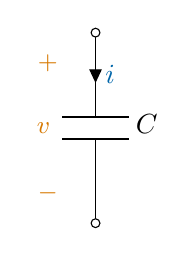
\begin{tikzpicture}[scale=1.1]\capDef\end{tikzpicture}
    \end{column}
    \begin{column}{0.68\textwidth}
      $q = C\,\Vcol{v}$, \quad $\Icol{i} = dq/dt$, \quad $C$ in farads (F)\\[12pt]
      \qbox{$\displaystyle \Icol{i(t)} = C\,\frac{d\Vcol{v}}{dt}
        \quad\iff\quad
        \Vcol{v(t)} = \Vcol{v(t_0)} + \frac{1}{C}\int_{t_0}^{t} \Icol{i(\tau)}\,d\tau$}
    \end{column}
  \end{columns}
  \vfill
  \pause
  \begin{itemize}\itemsep6pt
    \item $v$ constant (DC) $\Rightarrow$ $i = 0$: \ an \textbf{open circuit} in DC
    \item $v(t)$ depends on $v(t_0)$ \emph{and} all past current: \textbf{memory}
  \end{itemize}
  \vfill
\end{frame}

%==============================================================
\roadmapframe{5}

%--------------------------------------------------------------
\begin{frame}{Stored energy}
  \vfill
  \[
    \Pcol{w(t_0,t)} = \int_{t_0}^{t} v\,i\,d\tau = \int_{t_0}^{t} v\,C\frac{dv}{d\tau}\,d\tau
    = \tfrac12 C v(t)^2 - \tfrac12 C v(t_0)^2
  \]
  \pause
  Uncharged long ago, $v(-\infty) = 0$:
  \[ \qbox{$\Pcol{w(t)} = \tfrac12\,C\,\Vcol{v(t)}^2 \ \geq 0$} \]
  \pause
  \begin{itemize}\itemsep6pt
    \item Depends only on the present voltage
    \item Stored, not lost: it can be given back (passive element)
  \end{itemize}
  \vfill
\end{frame}

%--------------------------------------------------------------
\begin{frame}{Example 17.4: current and energy}
  \begin{columns}[c,onlytextwidth]
    \begin{column}{0.55\textwidth}
      $C = 2\F$, \ $\Vcol{v} = r(t) - r(t - 1)\V$.\\
      Find $\Icol{i(t)}$ and $\Pcol{w}$ for $t \geq 1$.\\
      What if $\Vcol{v} = u(t)\V$?\\[10pt]
      \onslide<2->{$\Icol{i} = 2\dfrac{d}{dt}\big[r(t) - r(t - 1)\big] = 2\big[u(t) - u(t - 1)\big]\A$\\[8pt]}
      \onslide<3->{$\Pcol{w} = \tfrac12 \cdot 2 \cdot 1^2 = 1\Jl$, \ no current for $t > 1$\\[8pt]}
      \onslide<4->{\qbox{$\Vcol{v} = u(t) \ \Rightarrow\ \Icol{i} = 2\,\delta(t)\A$}\\[4pt]
        \small A jump in $v$ needs an impulse of current.}
    \end{column}
    \begin{column}{0.43\textwidth}
      \centering
      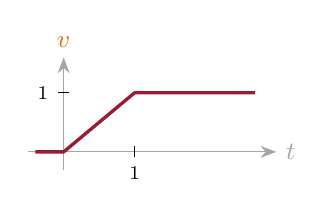
\begin{tikzpicture}[x=0.9cm,y=0.75cm]
        \tax{-0.5}{3.0}{-0.3}{1.6}{$t$}{$\Vcol{v}$}
        \draw[crv] (-0.4,0) -- (0,0) -- (1,1) -- (2.7,1); \xt{1}{$1$} \yt{1}{$1$}
      \end{tikzpicture}\\[4pt]
      \onslide<2->{%
      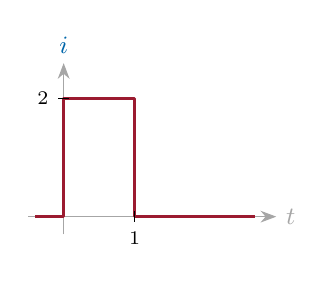
\begin{tikzpicture}[x=0.9cm,y=0.75cm]
        \tax{-0.5}{3.0}{-0.3}{2.6}{$t$}{$\Icol{i}$}
        \draw[crv] (-0.4,0) -- (0,0) -- (0,2) -- (1,2) -- (1,0) -- (2.7,0); \xt{1}{$1$} \yt{2}{$2$}
      \end{tikzpicture}}
    \end{column}
  \end{columns}
\end{frame}

%==============================================================
\roadmapframe{6}

%--------------------------------------------------------------
\begin{frame}{Three equivalent initial-condition models}
  \centering
  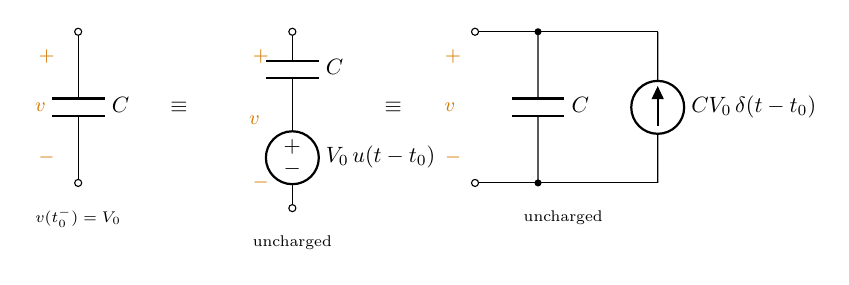
\begin{tikzpicture}[scale=0.8, transform shape]
    \begin{scope}\icModel{1}\end{scope}
    \node at (1.6,1.2) {$\equiv$};
    \begin{scope}[xshift=3.4cm]\icModel{2}\end{scope}
    \node at (5.0,1.2) {$\equiv$};
    \begin{scope}[xshift=6.3cm]\icModel{3}\end{scope}
  \end{tikzpicture}\\[4pt]
  \raggedright\small
  Equivalent: for $t > t_0$ the same $i$ gives the same $v$ at the terminals.\\[4pt]
  \onslide<2->{\textbf{1.} \ $v(t) = \Vo + \frac1C\int_{t_0^-}^{t} i\,d\tau$\\[2pt]}
  \onslide<3->{\textbf{2.} \ $v(t) = 0 + \frac1C\int_{t_0^-}^{t} i\,d\tau + \Vo$ \quad (the source adds $\Vo$)\\[2pt]}
  \onslide<4->{\textbf{3.} \ $v(t) = 0 + \frac1C\int_{t_0^-}^{t} \big[i + C\Vo\,\delta(\tau - t_0)\big]\,d\tau = \Vo + \frac1C\int_{t_0^-}^{t} i\,d\tau$\\[4pt]
    Model 2: series connections. \ Model 3: parallel connections.}
\end{frame}

%==============================================================
\roadmapframe{7}

%--------------------------------------------------------------
\begin{frame}{Parallel and series capacitors}
  \begin{columns}[t,onlytextwidth]
    \begin{column}{0.48\textwidth}
      \centering\textbf{Parallel}: same $v$\\[4pt]
      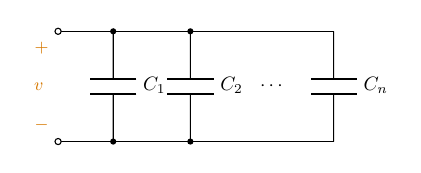
\begin{tikzpicture}[scale=0.7, transform shape]\capPar\end{tikzpicture}\\[4pt]
      \raggedright
      $i = C_1\dot v + \cdots + C_n\dot v$\\[6pt]
      \onslide<2->{\centering\qbox{$C_{eq} = C_1 + \cdots + C_n$}\\[4pt]
      \small $v_{eq}(t_0) = \Vo$}
    \end{column}
    \begin{column}{0.5\textwidth}
      \centering\textbf{Series}: same $i$\\[4pt]
      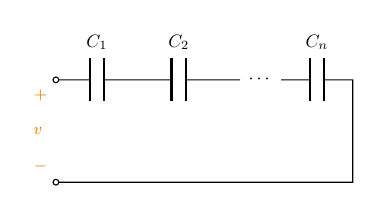
\begin{tikzpicture}[scale=0.65, transform shape]\capSer\end{tikzpicture}\\[4pt]
      \raggedright
      $v = v_1 + \cdots + v_n$, \ $v_k(t_0) = V_{k0}$\\[6pt]
      \onslide<3->{\centering\qbox{$\dfrac{1}{C_{eq}} = \dfrac{1}{C_1} + \cdots + \dfrac{1}{C_n}$}\\[4pt]
      \small $v_{eq}(t_0) = V_{10} + \cdots + V_{n0}$}
    \end{column}
  \end{columns}
  \vfill
  \onslide<4->{\centering\small Capacitors combine like conductances.}
\end{frame}

%==============================================================
\roadmapframe{8}

%--------------------------------------------------------------
\begin{frame}{Current division}
  \vfill
  \begin{columns}[c,onlytextwidth]
    \begin{column}{0.42\textwidth}
      \centering
      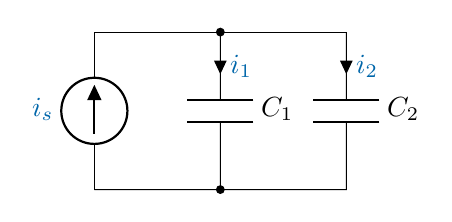
\begin{tikzpicture}[scale=1.0]\cdiv\end{tikzpicture}
    \end{column}
    \begin{column}{0.56\textwidth}
      Same voltage: \ $\dfrac{\Icol{i_1}}{C_1} = \dfrac{\Icol{i_2}}{C_2} = \dfrac{dv}{dt}$\\[8pt]
      KCL: \ $\Icol{i_1} + \Icol{i_2} = \Icol{i_s}$\\[10pt]
      \pause
      \qbox{$\Icol{i_1} = \dfrac{C_1}{C_1 + C_2}\,\Icol{i_s}, \qquad \Icol{i_2} = \dfrac{C_2}{C_1 + C_2}\,\Icol{i_s}$}\\[8pt]
      The larger capacitor takes the larger share.
    \end{column}
  \end{columns}
  \vfill
\end{frame}

%--------------------------------------------------------------
\begin{frame}{Voltage division}
  \begin{columns}[c,onlytextwidth]
    \begin{column}{0.38\textwidth}
      \centering
      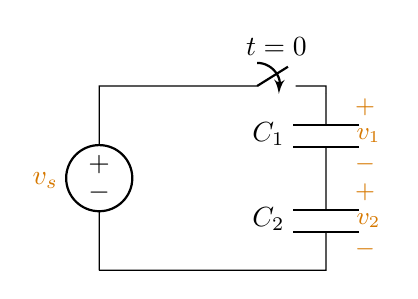
\begin{tikzpicture}[scale=0.9]\vdiv\end{tikzpicture}\\[6pt]
      \small $v_1(0^-) = V_{10}$, \ $v_2(0^-) = V_{20}$
    \end{column}
    \begin{column}{0.6\textwidth}
      Same current after $t = 0$:
      \[ \int_{0^-}^{t} i\,d\tau = C_1(v_1 - V_{10}) = C_2(v_2 - V_{20}) \]
      KVL: \ $v_1 + v_2 = \Vcol{v_s}$\\[4pt]
      \pause
      \[
        \Vcol{v_1} = \frac{C_2}{C_1 + C_2}\Vcol{v_s} + \frac{C_1V_{10} - C_2V_{20}}{C_1 + C_2}
      \]
      \pause
      \small $C_1 = 1\F$, $C_2 = 2\F$, $v_s = 6\V$:\\
      uncharged: $v_1 = 4\V$, $v_2 = 2\V$ \ (smaller $C$, larger $v$)\\
      $V_{10} = 3\V$: \ $v_1 = 5\V$, $v_2 = 1\V$
    \end{column}
  \end{columns}
\end{frame}

%==============================================================
\roadmapframe{9}

%--------------------------------------------------------------
\begin{frame}{From $0^-$ to $0^+$: is $\vC$ continuous?}
  \vfill
  \begin{itemize}\itemsep10pt
    \item Energy is finite: $\tfrac12 C\vC^2 < \infty$ \ $\Rightarrow$ \ $\vC$ is \textbf{bounded}
    \pause
    \item If $\iC$ is bounded on $[0^-, 0^+]$:
      \[ \vC(0^+) = \vC(0^-) + \frac1C\underbrace{\int_{0^-}^{0^+} \iC\,d\tau}_{0} = \vC(0^-) \]
    \pause
    \item Only an \emph{impulse} of current can make $\vC$ jump
  \end{itemize}
  \vfill
  \pause
  \centering
  \qbox{During $0^- < t < 0^+$: replace $C$ by a bounded voltage source $\vC(t)$}
  \vfill
\end{frame}

%--------------------------------------------------------------
\begin{frame}{Example 17.5: a step source}
  \begin{columns}[c,onlytextwidth]
    \begin{column}{0.45\textwidth}
      \centering
      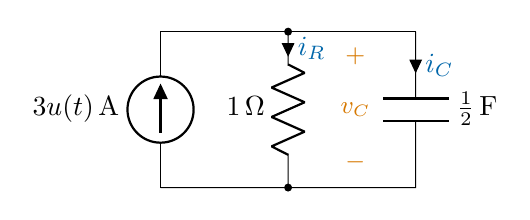
\begin{tikzpicture}[scale=0.9]\rcPar{$3u(t)\,\mathrm{A}$}{$1\ohm$}{$\tfrac12\F$}\end{tikzpicture}
    \end{column}
    \begin{column}{0.53\textwidth}
      Find $\vC(0^+)$, $\iR(0^+)$, $\iC(0^+)$ when\\
      (a) $\vC(0^-) = 0$, \quad (b) $\vC(0^-) = 4\V$.\\[8pt]
      \onslide<2->{\small $\iR = \vC/1$ bounded $\Rightarrow$ $\iC = 3u - \iR$ bounded\\
        $\Rightarrow$ \ $\vC(0^+) = \vC(0^-)$}
    \end{column}
  \end{columns}
  \vfill
  \onslide<3->{%
  \centering
  \renewcommand{\arraystretch}{1.3}
  \begin{tabular}{@{}lccc@{}}
    \toprule
    & $\vC(0^+)$ & $\iR(0^+) = \vC(0^+)/1$ & $\iC(0^+) = 3 - \iR(0^+)$\\
    \midrule
    (a) & $0$ & $0$ & $3\A$\\
    (b) & $4\V$ & $4\A$ & $-1\A$\\
    \bottomrule
  \end{tabular}\\[6pt]
  \small At the switching instant $C$ acts like a voltage source $\vC(0^-)$.}
  \vfill
\end{frame}

%==============================================================
\roadmapframe{10}

%--------------------------------------------------------------
\begin{frame}{Example 17.6: an impulse source}
  \begin{columns}[c,onlytextwidth]
    \begin{column}{0.45\textwidth}
      \centering
      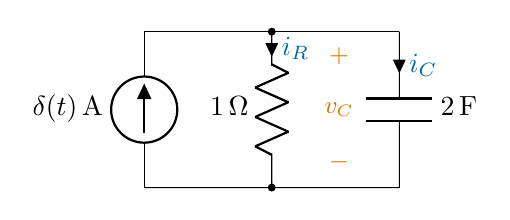
\begin{tikzpicture}[scale=0.9]\rcPar{$\delta(t)\,\mathrm{A}$}{$1\ohm$}{$2\F$}\end{tikzpicture}
    \end{column}
    \begin{column}{0.53\textwidth}
      $\vC(0^-) = 1\V$.\\
      Find $\vC(0^+)$, $\iR(0^+)$, $\iC(0^+)$.\\[8pt]
      \onslide<2->{\small $\iR = \vC/1$ bounded, \ $\iC = \delta(t) - \iR$}
    \end{column}
  \end{columns}
  \vfill
  \onslide<3->{%
  \[
    \vC(0^+) = 1 + \frac12\int_{0^-}^{0^+} \big[\delta - \iR\big]\,d\tau
    = 1 + \frac12 - 0 = 1.5\V
  \]}
  \onslide<4->{\centering $t = 0^+$: source is zero: \
    \qbox{$\iR(0^+) = 1.5\A, \quad \iC(0^+) = -1.5\A$}\\[6pt]}
  \onslide<5->{\small\centering Shortcut: replace $C$ by a short; the impulse flows only through the short.}
  \vfill
\end{frame}

%==============================================================
\roadmapframe{11}

%--------------------------------------------------------------
\begin{frame}{Example 17.7: an RC circuit discharging}
  \begin{columns}[c,onlytextwidth]
    \begin{column}{0.4\textwidth}
      \centering
      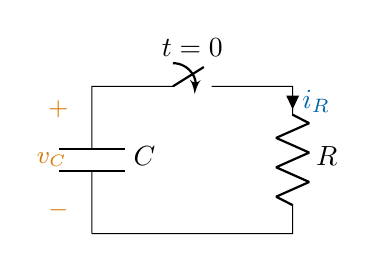
\begin{tikzpicture}[scale=0.85]\rcDis\end{tikzpicture}\\[4pt]
      \small $\vC(0^-) = \Vo$
    \end{column}
    \begin{column}{0.58\textwidth}
      \onslide<2->{$\vC(0^+) = \Vo$ \ (bounded current)\\[6pt]}
      \onslide<3->{$t > 0$: \ $C\dfrac{d\vC}{dt} = -\dfrac{\vC}{R}$\\[6pt]}
      \onslide<4->{\qbox{$\vC(t) = \Vo\,e^{-t/RC}, \quad \iR(t) = \dfrac{\Vo}{R}\,e^{-t/RC}$}}
    \end{column}
  \end{columns}
  \vfill
  \onslide<4->{%
  \centering
  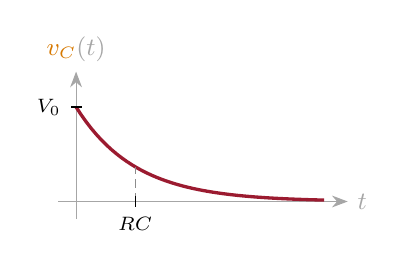
\begin{tikzpicture}[x=0.75cm,y=0.75cm]
    \tax{-0.3}{4.6}{-0.3}{2.2}{$t$}{$\vC(t)$}
    \draw[crv, domain=0:4.2, samples=50] plot (\x, {1.6*exp(-\x)});
    \yt{1.6}{$\Vo$} \draw[gdash] (1,0) -- (1,{1.6*exp(-1)}); \xt{1}{$RC$}
  \end{tikzpicture}\hspace{1cm}
  \begin{minipage}[b]{0.45\textwidth}\small
    \onslide<5->{$\Pcol{w_C(0,t)} = \tfrac12 C\Vo^2\big[e^{-2t/RC} - 1\big] < 0$\\[4pt]
    $\Pcol{w_R(0,t)} = \tfrac12 C\Vo^2\big[1 - e^{-2t/RC}\big]$\\[4pt]
    $\Pcol{w_C + w_R} = 0$: all stored energy becomes heat.}
  \end{minipage}}
\end{frame}

%==============================================================
\roadmapframe{12}

%--------------------------------------------------------------
\begin{frame}{Example 17.8: two capacitors and a switch}
  \begin{columns}[c,onlytextwidth]
    \begin{column}{0.42\textwidth}
      \centering
      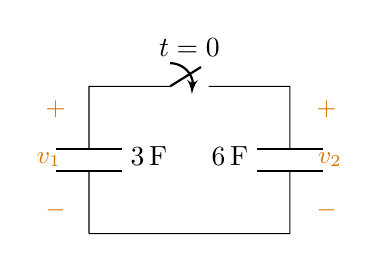
\begin{tikzpicture}[scale=0.85]\twoCap\end{tikzpicture}\\[4pt]
      \small $v_1(0^-) = 0$, \ $v_2(0^-) = 3\V$
    \end{column}
    \begin{column}{0.56\textwidth}
      Find $v_1(0^+)$ and the energy before and after.\\[8pt]
      \onslide<2->{Charge: $i_1 + i_2 = 0$ \ $\Rightarrow$ \ $3(v_1 - 0) + 6(v_2 - 3) = 0$\\[4pt]}
      \onslide<3->{KVL: $v_1 = v_2$ \ $\Rightarrow$ \ \qbox{$v_1(0^+) = v_2(0^+) = 2\V$}\\[4pt]
        \small The voltages \emph{jump}: an impulse of current flows.}
    \end{column}
  \end{columns}
  \vfill
  \onslide<4->{\centering
    $\Pcol{E(0^-)} = \tfrac12\cdot 6\cdot 3^2 = 27\Jl$, \qquad
    $\Pcol{E(0^+)} = \tfrac12(3 + 6)\cdot 2^2 = 18\Jl$\\[6pt]}
  \onslide<5->{\centering $9\Jl$ is missing. Where did it go?}
  \vfill
\end{frame}

%--------------------------------------------------------------
\begin{frame}{The missing energy}
  \vfill
  \begin{itemize}\itemsep8pt
    \item A real switch has resistance $R$
    \item Series capacitors: $C_s = \dfrac{3\cdot 6}{3 + 6} = 2\F$, initial difference $3\V$
    \pause
    \item As in Example 17.7: \ $i = \dfrac{3}{R}\,e^{-t/2R}$
    \[
      \Pcol{w_R} = \int_0^{\infty} R\left(\frac{3}{R}\right)^2 e^{-t/R}\,dt = \frac{9}{R}\cdot R = 9\Jl
    \]
  \end{itemize}
  \pause
  \centering
  \qbox{$9\Jl$ is lost in the switch, \emph{whatever} $R$ is}\\[6pt]
  \small $R \to 0$: the current becomes an impulse, the loss stays $9\Jl$.
  \vfill
\end{frame}

%--------------------------------------------------------------
\begin{frame}{Summary}
  \small
  \renewcommand{\arraystretch}{1.35}
  \begin{tabular}{@{}p{0.22\textwidth}p{0.72\textwidth}@{}}
    \toprule
    step, ramp, impulse & $\int \delta = u$, \ $\int u = r$; a jump $a$ at $t_0$ gives $a\,\delta(t - t_0)$\\
    sifting & $f(t)\,\delta(t - t_0) = f(t_0)\,\delta(t - t_0)$\\
    capacitor & $i = C\,dv/dt$; open circuit in DC; memory\\
    energy & $w = \tfrac12 Cv^2 \geq 0$: stored, not lost\\
    initial condition & charged $C$ $\equiv$ uncharged $C$ + step source $\equiv$ uncharged $C$ $\|$ impulse\\
    connections & parallel $\sum C_k$; series $1/C_{eq} = \sum 1/C_k$\\
    $0^-$ to $0^+$ & bounded $\iC$ $\Rightarrow$ $\vC$ continuous; only an impulse makes it jump\\
    RC discharge & $\vC = \Vo e^{-t/RC}$; all stored energy ends in $R$\\
    \bottomrule
  \end{tabular}
\end{frame}

\end{document}
